
\chapter{Task-Aware Online Model Search with Misspecified Model Classes}
\label{CHA:TAML}

\epigraph{\textit{More work is needed before planning with learned
    models can be effective. Environment models should be
    constructed judiciously with regard to both their states and
    dynamics with the goal of optimizing the planning process.}}{Rich
  Sutton and Andrew Barto (2018)}

The algorithms presented in this thesis, so
far, have not required any updates to the dynamics of the model. In
contrast, most existing methods in the literature, such
as~\cite{DBLP:journals/ml/KearnsS02, DBLP:journals/jmlr/BrafmanT02,
  DBLP:conf/atal/JongS07,
  DBLP:journals/pami/DeisenrothFR15, DBLP:conf/icml/AbbeelQN06,
  DBLP:conf/aaai/Jiang18, rastogi2018sample}, use experience
acquired from executions to update the dynamics of the model or learn
a model from scratch.
Chapters~\ref{CHA:CMAX} and~\ref{CHA:CMAXPP} have
argued that updating the dynamics of the model requires a large amount
of experience in large state spaces and can be at the expense of
completing the task. While this is generally true, there are major
advantages of updating the dynamics of the model, especially in
domains where it
is feasible to do it online, as it allows the planner to compute
solutions that exploit the true dynamics and potentially result in
solutions with very low costs. Furthermore even in application domains
where we require a large amount of experience to update the model,
the improvement in task performance from planning on a more accurate
model can outweigh the executions wasted to learn true dynamics. For
example, there might be regions in the state space where updating the
dynamics of the model can be done efficiently while in other regions
we can resort to methods that update the behavior of planner such as
\cmax{} and \cmaxpp{}. This motivates a trade-off between both sets of
approaches and understanding this trade-off can result in intelligent
use of online experience to achieve efficient planning and
execution.

This chapter presents \taml{} an online model search algorithm that updates
the dynamics of the model to directly optimize task performance,
rather than optimizing prediction error that is commonly done in
existing works. This allows \taml{} to use misspecified model classes,
where none of the models are able to capture the true dynamics
accurately, and still improve the task performance by updating the
model dynamics. This chapter is based on ongoing work.

\section{Problem Setup}
\label{sec:problem-setup-1}

We consider the deterministic shortest path problem represented using
the tuple $M = (\statespace, \actionspace, \goalspace, f, c)$ where
$\statespace$ is the state space, $\actionspace$ is the action space,
$\goalspace \subset \statespace$ is the set of goals that we are
interested in reaching, $f: \statespace \times \actionspace
\rightarrow \statespace$ is the deterministic dynamics, and $c:
\statespace \times \actionspace \rightarrow [0, 1]$ is the cost
function. We assume that any goal state $g \in \goalspace$ is a
cost-free termination state. The objective of the shortest path
problem is to find the least-cost path from a given start state $s_1
\in \statespace$ to any goal state $g \in \goalspace$ in $M$. As is
typical in shortest path problems, we assume that there exists at
least one path from each state $s \in \statespace$ to one of the goal
states in $\goalspace$.

In this work, we focus on environments $M$ with unknown transition
dynamics $f$ and known cost function $c$. Instead we have access to a
dynamical model class 
$\mathcal{F} = \{\hat{f}_\theta: \statespace \times \actionspace \rightarrow
\statespace \}$ that is parameterized by $\theta \in \Theta$. We do
not require that $f \in \mathcal{F}$, i.e. the model class
$\mathcal{F}$ can be misspecified. This is usually true in real-world
domains where the true dynamics can be time-varying and arbitrarily
complex. Even in domains where the dynamics are not complex, we might
desire to chose a small model class to achieve computational
efficiency for methods to run in real-time. The robot gathers
knowledge of the true dynamics over a single trajectory in the
environment, and does not have access to any resets, ruling out any
episodic approach.

We assume we have access to a planner $P$ that when given a dynamical
model $\hat{f}_\theta$ results in a policy $\pi_\theta: \statespace \rightarrow
\actionspace$ that optimizes 
the cost-to-go according to the cost function $c$ and transition
dynamics $\hat{f}_\theta$. Note that we do not require $P$ to be an
optimal planner. We will use the notation $V_\theta^{\pi_\theta}(s)$ to denote
the cost-to-go (or state value function) from state $s$ using policy
$\pi_\theta$ under the transition 
dynamics given by $\hat{f}_\theta \in \mathcal{F}$. To denote the
cost-to-go of any policy $\pi_\theta$\footnote{Note that we use the
  same parameterization $\theta$ for both policies and dynamical
  models as we only consider the class of policies that result from
  applying the planner $P$ on the dynamical model class
  $\mathcal{F}$.} in $M$ under the true dynamics $f$, we use the
notation $V^{\pi_\theta}$. Similarly, we will use the notation
$Q_\theta^{\pi_\theta}(s, a)$ and $Q^{\pi_\theta}(s, a)$ to denote the
state-action value function (or cost-to-go after executing action $a$
in state $s$) in the model $\hat{f}_\theta$ and in $M$ respectively.

Our method, \taml{}, relies crucially on having access to an
optimistic dynamical model $\fopt: \statespace \times \actionspace
\rightarrow \statespace$. An optimistic dynamical model satisfies
the following assumption:
\begin{assumption}
  For any policy $\pi$, the cost-to-go $V^\pi_\opt$ using the dynamics
  $\fopt$ underestimates the cost-to-go $V^\pi$ using the true
  dynamics $f$ at all states, i.e. $V^\pi_\opt(s) \leq V^\pi(s)$ for
  all $s \in \statespace$.
  \label{assumption:taml-optimistic}
\end{assumption}
where we use the notation $V_\opt^\pi$ to denote the cost-to-go of
policy $\pi$ under the transition dynamics of the optimistic model
$\fopt$.

\section{Relevant Prior Work}
\label{sec:prior-work}

\subsection{Maximum Likelihood Model Learning}
\label{sec:maxim-likel-model}

Most of the existing model learning methods use a maximum-likelihood
estimation objective (MLE) that optimizes prediction error to choose the best
model $\hat{f}_\theta$ among the class $\mathcal{F}$. Given a set of
transitions obtained from execution in $M$, $\mathcal{D} = \{(s_i, a_i,
s_{i+1})\}_{i=1}^N$ where $s_i \in \statespace, a_i \in \actionspace$
and $s_{i+1} = f(s_i, a_i)$ we construct a loss function 
given as follows:
\begin{equation}
  \label{eq:21}
  \mathcal{L}^\mle(\theta) = \frac{1}{N} \sum_{i=1}^{N} (s_{i+1} -
  \hat{f}_\theta(s_i, a_i))^2
\end{equation}
While we deal with deterministic dynamics in this work, in the
stochastic setting the above L2 norm prediction error can be derived
from maximum likelihood estimator by modeling the stochastic one-step
transition dynamics using a gaussian distribution.

Once we find $\theta^\mle = \arg\min_{\theta}
\mathcal{L}_\mle(\theta)$, we use the planner $P$ to find the
corresponding policy $\pi_{\theta^\mle}$ that is used for future
executions in $M$. There are some subtleties that are required in
these approaches where we require that the data $\mathcal{D}$ is
collected using a sufficiently exploratory policy to ensure good
coverage. We will refer the curious reader to these works to
understand these subtleties.

\subsection{Reward Based Model Search}
\label{sec:reward-based-model}

\cite{DBLP:conf/icra/JosephGRHR13} presented an offline model search
approach RBMS that eschews maximum likelihood learning and directly
optimizes the cost-to-go in $M$. Similar to our work, they treat the
dynamical model class as a parameterization of the policy (using
planner $P$) and search for $\theta^\rbms$ that achieves the least
cumulative cost using a gradient descent procedure as follows:
\begin{equation}
  \label{eq:22}
  \theta = \theta - \alpha \frac{\partial
    V^{\pi_{\theta}}(s_1)}{\partial {\theta}}
\end{equation}
where $\alpha > 0$ is the stepsize.

To compute the update in \eqref{eq:22} we require gradient of
cost-to-go of policy $\pi_{\theta}$ in $M$ w.r.t ${\theta}$,
i.e. $\frac{\partial
    V^{\pi_{\theta}}(s_1)}{\partial {\theta}}$ which is
  extremely difficult to compute as the operation that results in
  $V^{\pi_{\theta}}$ from ${\theta}$ can be highly
  nonlinear. \cite{DBLP:conf/icra/JosephGRHR13} sidestep this
  difficulty by using a zeroth-order estimate of the gradient obtained
  from evaluating $V^{\pi_{\theta}}$ for small perturbations of
  ${\theta}$.

  Given a policy $\pi_{{\theta}}$, RBMS evaluates $V^{\pi_{\theta}}$
  in an off-policy fashion using offline collected dataset
  $\mathcal{D} = \{(s_i, a_i, s_{i+1})\}_{i=1}^N$ which consists
  of transitions in $M$ collected by executing an exploratory policy
  different from $\pi_\theta$. For a fixed horizon length $H$,
  $V^{\pi_\theta}$ is computed by starting at $s_1$ and sequentially
  adds transitions such that at time $t$ when the robot is at state
  $\tilde{s}$, the next transition is $(s_t, a_t, s_{t+1}) =
  \arg\min_{(s, a, s') \in \mathcal{D}} \Delta((\tilde{s},
  \pi_\theta(\tilde{s})), (s, a))$ where $\Delta$ is a user-defined
  distance metric in state-action space. Note that each transition in
  $\mathcal{D}$ can only be used once, and the episode is terminated
  after $H$ steps. The cumulative cost of the resulting episode is
  used as a proxy for $V^{\pi_\theta}$.

  \begin{algorithm}[t]
    \caption{Model Search Using Derivative-Free Optimization~\cite{DBLP:conf/icra/JosephGRHR13}}
    \begin{algorithmic}[1]
      \Procedure{$\mathsf{MODELSEARCH}$}{$\mathcal{D}$}
      \State Initial perturbation $\delta^{init}$,
        minimum perturbation $\delta^{min}$, start parameters $\theta$,
      Initial state $s_1$, $\delta \leftarrow \delta^{init}$, planner $P$
      \While {$\delta > \delta^{min}$}
      \For {each dimension of $\Theta$}
      \While {True}
      \State Compute $\{\pi_{\theta^-}, \pi_\theta, \pi_{\theta^+}\}
      \leftarrow \{P(\hat{f}_{\theta - \delta}), P(\hat{f}_{\theta}),
      P(\hat{f}_{\theta + \delta})\}$
      \State Evaluate $\{V^{\pi_{\theta^-}}, V^{\pi_\theta},
      V^{\pi_{\theta^+}}\}$ \label{line:evaluation}
      \If {$\min(V^{\pi_{\theta^-}}(s_1), V^{\pi_{\theta^+}}(s_1)) >
        V^{\pi_\theta}(s_1)$}
      \State \textbf{break}
      \EndIf
      \If {$V^{\pi_{\theta^-}}(s_1) < V^{\pi_{\theta^+}}(s_1)$}
      \State $\theta \leftarrow \theta - \delta$
      \Else
      \State $\theta \leftarrow \theta + \delta$
      \EndIf
      \EndWhile
      \EndFor
      \State $\delta \leftarrow \frac{\delta}{2}$
      \EndWhile \\
      \Return{$\theta$}
      \EndProcedure
    \end{algorithmic}
    \label{alg:hill-climbing}
  \end{algorithm}

  Given this estimate of $V^{\pi_\theta}$ for any $\theta$, RBMS
  performs a hill climbing procedure (shown in
  Algorithm~\ref{alg:hill-climbing}) by perturbing $\theta$ locally 
  and repeating until we reach a local minima at which it returns the
  $\theta^\rbms$ found. Since, the objective optimized
  $V^{\pi_\theta}$ directly corresponds to task performance, RBMS is
  able to find the best performing model in a misspecified model class
  that achieves good task performance.

While RBMS is a task-aware model search procedure, it is an offline
method that requires the dataset $\mathcal{D}$ to have good
coverage. As we show in our experiments, the online version of RBMS,
where we are collecting the dataset $\mathcal{D}$ online while
executing policies found by RBMS in $M$, can result in a very poor
performance as the dataset $\mathcal{D}$ will not have a good coverage
and can result in a highly inaccurate estimate of $V^{\pi_\theta}$. We
will show that our approach \taml{} sidesteps this by falling back on
the optimistic dynamical model $\fopt$ in state-action space regions
where online data $\mathcal{D}$ does not have good coverage.

\section{Approach}
\label{sec:approach-2}

Our approach \taml{} builds upon RBMS by extending to the online
setting where policy execution and model updates are interleaved. In
addition to the online setting, \taml{} also uses a more informative
cost-to-go evaluation procedure that allows it to use data collected
online that might not have good coverage of state-action space while
still improving the task performance of the policy. We will first
describe the online setting and present the framework in
Section~\ref{sec:online-setting}. Subsequently in
Section~\ref{sec:evaluation}, we will explain our 
novel off-policy evaluation procedure that uses the optimistic model in
state-action space regions where we do not have good data coverage.

\subsection{Online Model Search}
\label{sec:online-setting}
Extending RBMS to the online setting requires us to specify how the
data is collected, and once the data is collected how the policy is
updated. The online setting we consider is the deterministic shortest
path problem described in Section~\ref{sec:problem-setup-1}, where the
robot has no access to resets and can gain knowledge about the true
dynamics of $M$ through a single trajectory.

\begin{algorithm}[t]
  \caption{Online Model Search Framework}
  \begin{algorithmic}[1]
    \Require{Initial state $s_1$, Planner $P$, Initial Model $\theta$,
      Dataset $\mathcal{D} = \{\}$, Model update frequency $\nu \in \mathbb{Z}$}
    \State $t \leftarrow 1$, $\pi_\theta \leftarrow P(\hat{f}_\theta)$
    \While {$s_t \notin \goalspace$}
    \State Compute $a_t \leftarrow \pi_\theta(s_t)$
    \State Execute $a_t$ in $M$ to get $s_{t+1} = f(s_t, a_t)$
    \State Update $\mathcal{D} = \mathcal{D} \cup \{(s_t, a_t,
    s_{t+1})\}$
    \If{$t$ is a multiple of $\nu$}
    \State Update $\theta \leftarrow
    \mathsf{MODELSEARCH}(\mathcal{D})$
    \State Update $\pi_\theta \leftarrow P(\hat{f}_\theta)$
    \EndIf
    \EndWhile
  \end{algorithmic}
  \label{alg:online-model-search}
\end{algorithm}

The online model search framework is given in
Algorithm~\ref{alg:online-model-search}. Starting from the initial
state, the robot executes the policy computed by the planner using the
dynamical model $\hat{f}_\theta$ where $\theta$ is the
parameterization of the initial model. For each execution in $M$ using
the policy $\pi_\theta$, we store the resulting transition in the
dataset $\mathcal{D}$. Once every $\nu$ executions, we use the data
collected so far, and run a model search procedure to pick a new
$\theta$ and update the policy using the planner $P$. This process is
repeated until the robot reaches the goal.

Observe that we collect the dataset $\mathcal{D}$ using the current
policy that is used for execution. Note that this is in contrast to the 
offline setting where we have a fixed dataset that is given to us
prior to execution that is collected by executing a fixed exploratory
policy. In the online setting, as the policy changes it results in a
different set of states visited thereby changing the dataset
$\mathcal{D}$. Furthermore, due to the lack of resets we obtain more
data in regions where the current policy spends more executions. These
characteristics of the online dataset $\mathcal{D}$ pose challenges to
maximum likelihood model learning methods and offline model search
methods like RBMS.

Due to the non-stationary nature of the dataset $\mathcal{D}$, maximum
likelihood methods find a model that best predicts the true dynamics
for states that were visited during execution, and can have terrible
prediction everywhere else. This can result in a bad policy that does
not make any progress towards the goal. Meanwhile offline methods like
RBMS rely on off-policy evaluation procedures (such as the one
described in Section~\ref{sec:reward-based-model}) that solely rely on
the dataset $\mathcal{D}$. Due to the lack of good coverage in the
dataset, these evaluation procedures can be highly inaccurate and
pessimistic resulting in convergence to poor policies when used in
model search. Our approach \taml{} builds upon RBMS by using an
optimistic off-policy evaluation procedure that is described in the
next section.

\subsection{Optimistic Off-Policy Evaluation}
\label{sec:evaluation}

Given a policy $\pi_\theta$ and dataset $\mathcal{D}$ of transitions
executed in $M$, our goal is to estimate the cost-to-go
$V^{\pi_\theta}$ of the policy in $M$. RBMS estimates this by solely
using the dataset $\mathcal{D}$, while our approach \taml{} relies on
$\mathcal{D}$ only in regions where it has good coverage and falls
back on the optimistic dynamical model $\fopt$ elsewhere. To determine
if the dataset has good coverage for a state-action pair $(s, a)$, we
compute the distance to the closest state-action pair in the dataset
$\mathcal{D}$. A user-defined distance threshold $\mu$ determines
whether we use the transition in the dataset to obtain the successor
or to fall back on the optimistic model $\fopt$. The
optimistic off-policy evaluation procedure is given in
Algorithm~\ref{alg:evaluation}.

\begin{algorithm}[t]
  \caption{Optimistic Off-Policy Evaluation}
  \begin{algorithmic}[1]
    \Require{Policy $\pi_\theta$, Dataset $\mathcal{D}$, start state
      $s_1$, horizon $H$, Distance metric $\Delta$, Distance threshold
      $\mu \geq 0$}
    \State Initialize $\tilde{s} \leftarrow s_1$, $\hat{V}^{\pi_\theta}(s_1)
    \leftarrow 0$
    \For{$t = 1$ to $H$}
    \State Compute $\tilde{a} \leftarrow \pi_\theta(\tilde{s})$
    \State Find $(s_t, a_t, s_{t+1}) \leftarrow \arg\min_{(s, a, s')
      \in \mathcal{D}} \Delta((\tilde{s}, \tilde{a}), (s, a))$
    \If{$\Delta((\tilde{s}, \tilde{a}), (s_t, a_t)) \leq \mu$}
    \State $\mathcal{D} \leftarrow \mathcal{D} \setminus (s_t, a_t,
    s_{t+1})$
    \Else
    \State Compute $s_{t+1} \leftarrow \fopt(s_t, a_t)$
    \EndIf
    \State $\hat{V}^{\pi_\theta}(s_1) \leftarrow  \hat{V}^{\pi_\theta}(s_1) + c(s_t, a_t)$,
    $\tilde{s} \leftarrow s_{t+1}$
    \If{$\tilde{s} \in \goalspace$}
    \State \textbf{break}
    \EndIf
    \EndFor \\
    \Return{$\hat{V}^{\pi_\theta}(s_1)$}
  \end{algorithmic}
  \label{alg:evaluation}
\end{algorithm}

Starting from the initial state $s_1$, we compute the action computed
by the policy and find the closest state-action pair from the dataset
$\mathcal{D}$ as measured by the distance metric $\Delta$. If the
closest state-action pair is closer than $\mu$, then we assign the
successor of the closest state-action pair as the next state and
remove it from the dataset $\mathcal{D}$. Else, we query
the optimistic model $\fopt$ to obtain the next state. Our evaluation
procedure differs from the evaluation procedure used in RBMS in that
we use $\mu$ to switch between using dataset $\mathcal{D}$ for
state-action regions with good coverage and using optimistic model
$\fopt$ elsewhere.

Combining all the components so far, \taml{} uses the novel optimistic
off-policy evaluation procedure from Algorithm~\ref{alg:evaluation} in
Line~\ref{line:evaluation} of Algorithm~\ref{alg:hill-climbing}. The
resulting $\mathsf{MODELSEARCH}$ procedure is used in the online model
search framework presented in Algorithm~\ref{alg:online-model-search}.

\section{Theoretical Guarantees}
\label{sec:theor-guar}

Our first guarantee shows that using optimistic off-policy evaluation
as done in Algorithm~\ref{alg:evaluation} always results in a
cost-to-go estimate that is not too pessimistic. In other words, we
have
\begin{theorem}
  If the state-action value function $Q^{\pi_\theta}$ is $L$-lipschitz
  under the 
  distance metric $\Delta$ for any policy $\pi_\theta$, then we have
  that the estimate $\hat{V}^{\pi_\theta}$ satsfies
  \begin{equation}
    \label{eq:25}
    \hat{V}^{\pi_\theta} \leq V^{\pi_\theta} + LH\mu
  \end{equation}
  where $H$ is the horizon, and $V^{\pi_\theta}$ is the true
  cost-to-go of the policy $\pi_\theta$ in $M$.
  \label{theorem:lipschitz}
\end{theorem}
\begin{proof}[Proof Sketch]
  Observe that if we never use any transition in the dataset
  $\mathcal{D}$, then we completely rely on the optimistic model
  $\fopt$ for evaluation which by definition results in a cost-to-go
  estimate $\hat{V}^{\pi_\theta}$ that is optimistic. Now, let's say
  we use a transition $(s, a, s') \in \mathcal{D}$ to evaluate the
  cost-to-go of $(\tilde{s}, \tilde{a})$, then we have that
  \begin{align*}
    Q^{\pi_\theta}(s, a) - Q^{\pi_\theta}(\tilde{s}, \tilde{a}) &\leq L\Delta((\tilde{s},
                              \tilde{a}), (s, a)) \\
    &\leq L\mu
  \end{align*}
  Thus, we can introduce a pessimistic error of at most $L\mu$
  everytime we use a transition from $\mathcal{D}$. In the worst case,
  we use $H$ transitions from $\mathcal{D}$, and thus our resulting
  cost-to-go estimate $\hat{V}^{\pi_\theta}$ can overestimate the true
  cost-to-go $V^{\pi_\theta}$ by $LH\mu$.
\end{proof}

The above guarantee highlights the advantage of \taml{} using an
optimistic off-policy evaluation method. By not being severely
pessimistic, \taml{} never discounts a policy before obtaining enough
data to do it with certainty. This allows \taml{} to always be
optimistic and not rely on inaccurate pessimistic value estimates. The
potential downside of this is that we might not be exploiting the
dataset $\mathcal{D}$ completely, but turns out collecting more data
is not as harmful as switching to a much worse policy based on
inaccurate evaluation as evidenced in our experiments.

We can also provide a task-completeness guarantee for \taml{} in small
state-action spaces (where we can set $\mu = 0$) when given access to
unlimited computation (allowing us to solve the hill-climbing
procedure in Algorithm~\ref{alg:hill-climbing} a large number of times
to reach global minima) which is stated as follows:
\begin{theorem}[Task Completeness]
  In small state-action spaces \taml{}, given
  access to unlimited computation, is guaranteed to reach a goal state
  if there exists at least a single model in the model class
  $\mathcal{F}$ that is good enough to result in a policy that can
  reach the goal in $M$.
  \label{theorem:toms-completeness}
\end{theorem}
\begin{proof}[Proof Sketch]
  From Theorem~\ref{theorem:lipschitz} we have that when we set $\mu =
  0$, the resulting cost-to-go estimates are always optimistic. Thus,
  as the robot collects more data it either reaches the goal or
  collects enough data to get the true cost-to-go estimate. In the
  latter case, since we are performing exact global optimization,
  \taml{} is guaranteed to find the best model in the model class that
  minimizes the true cost-to-go. As long as this best model results in
  a policy that can reach the goal, \taml{} will also reach the goal
  by picking this model and using its corresponding policy.
\end{proof}

\section{Experiments}
\label{sec:experiments-1}

We compare \taml{} against RBMS, maximum likelihood model learning
(MLE) and \cmax{} on a variant of the standard mountain car
domain. This variant 
was first introduced in~\cite{DBLP:conf/icra/JosephGRHR13}. In this
variant of the classic mountain car (shown in
Figure~\ref{fig:mountaincar}), there is a rock (shown in red in the
Figure) which causes the car to decrease its speed by $c$ whenever the
car moves across the rock in either direction. The dynamics of
mountain car are specified as follows:
\begin{align*}
  x_{t+1} &= x_t + \dot{x}_t \\
  \dot{x}_{t+1} &= \dot{x}_t + a + \theta_1\cos(\theta_2x_t)
\end{align*}
where $a \in \{-0.001, 0.001\}$ is the action executed. We use a
uniform discretization of $x$ and $\dot{x}$ with a $500 \times 250$
grid. The model class used by all approaches is $\mathcal{F} =
\{(\theta_1, \theta_2) | \theta_1, \theta_2 \in \reals\}$. The
environment $M$ (as shown in Figure~\ref{fig:mountaincar}) uses
$\theta_1 = -0.0025$ and $\theta_2 = 3$ for the dynamics everywhere
except at the rock where the velocity dynamics differ. Therefore,
increasing $c$ corresponds to the model class $\mathcal{F}$ becoming
increasingly misspecified. The initial position for the car is randomized
across each trial by sampling uniformly at random from
$[\frac{-\pi}{6} - 0.1, \frac{-\pi}{6}+0.1]$ with the initial velocity
set to $0$. The rock is placed at $x = 0.25$ for all the trials with
the goal at $x = 0.5$. The cost is $1$ everywhere except at the goal
where it is $0$. We use the distance function $\Delta$ given by,
\begin{equation}
  \label{eq:24}
  \Delta((s, a), (s', a')) =
  \begin{cases}
    \sum_{d=1}^D \frac{|s^d - s'^d|}{s^d_{max} - s^d_{min}} & \text{if
    } a = a' \\
    \infty & \text{otherwise}
  \end{cases}
\end{equation}
For \taml{}, we use the threshold $\mu = 0.01$ as specified by the
above distance metric.

\begin{figure}[t]
  \centering
  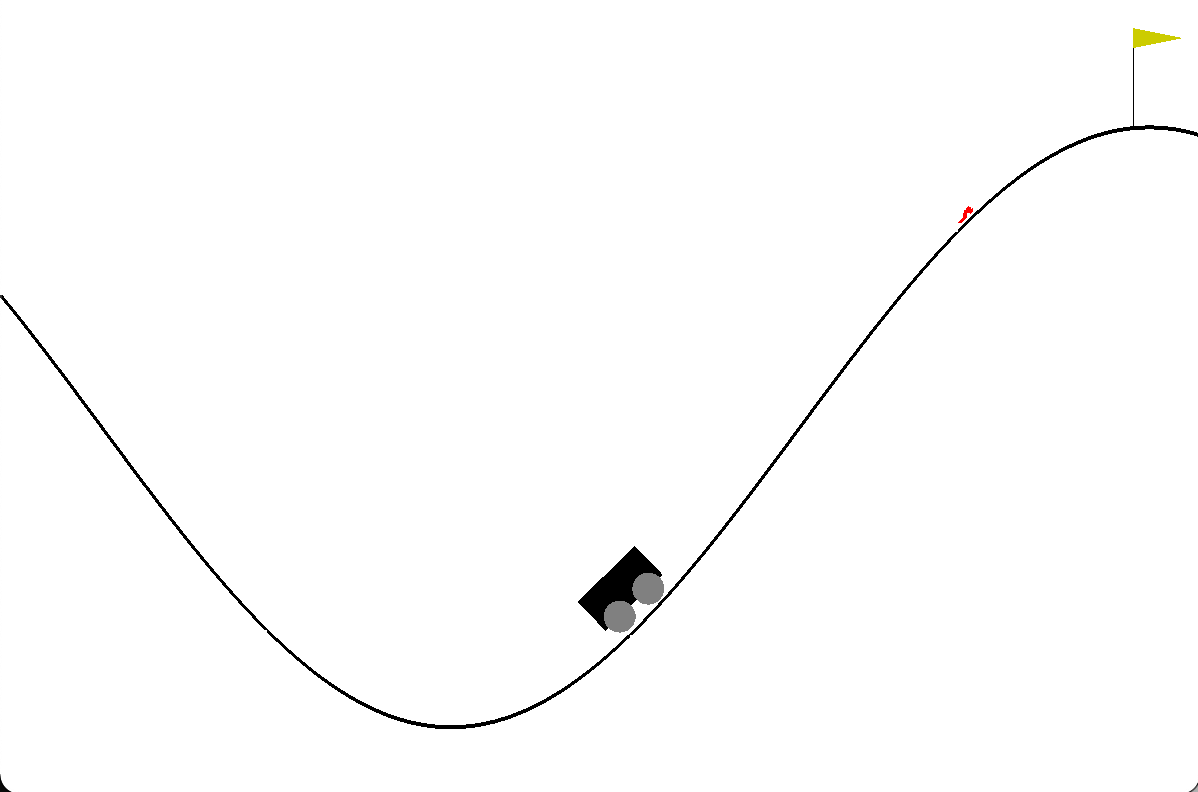
\includegraphics[width=0.5\linewidth]{figures/taml/mountaincar.png}
  \caption{Mountain Car Domain with Rock}
  \label{fig:mountaincar}
\end{figure}

Through our experiments, we would like to answer the following two
questions:
\begin{enumerate}
\item \textit{Does using \taml{} help in reaching the goal quickly
    despite lack of knowledge of the rock dynamics and the model class
    being misspecified?}
\item \textit{Does using optimistic model for off-policy evaluation
    help in achieving better value estimates that are useful for
    reaching the goal quickly?}
\end{enumerate}

\begin{figure}[t]
  \centering
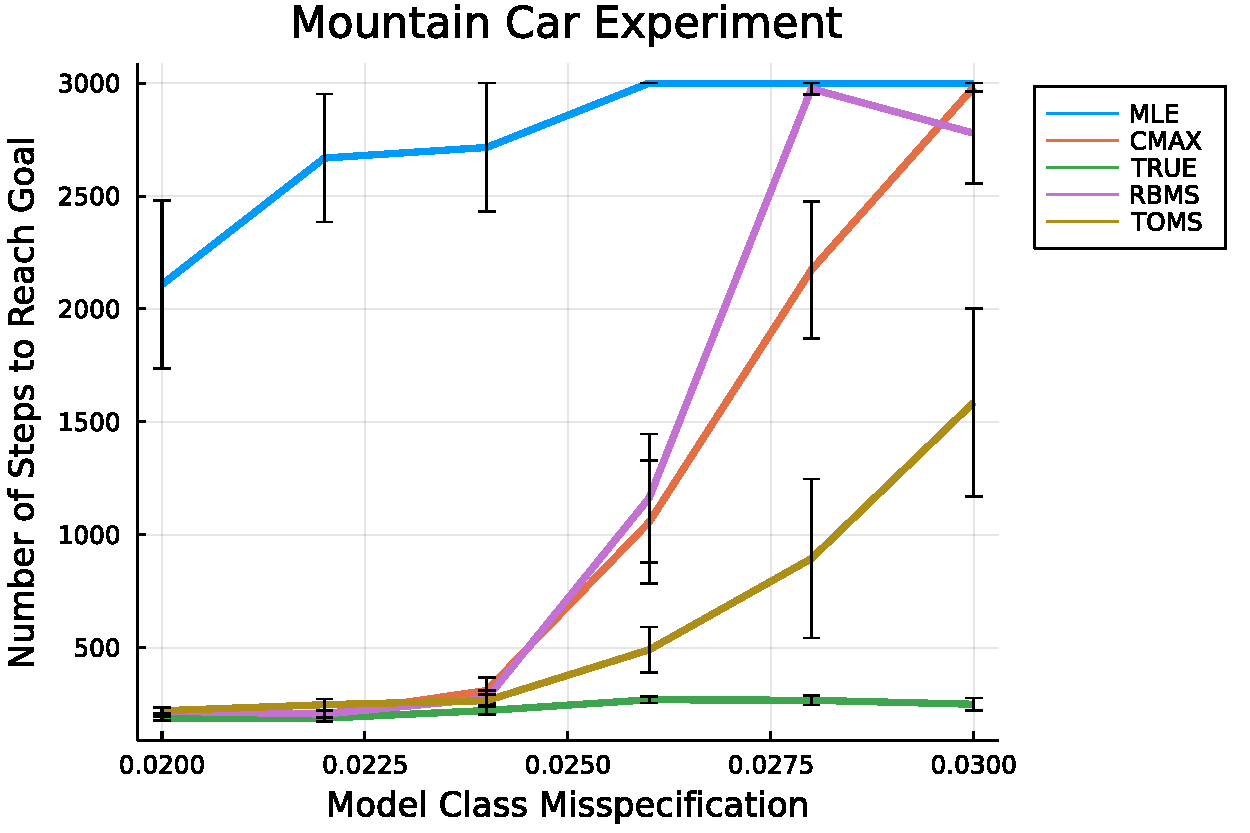
\includegraphics[width=0.5\linewidth]{figures/taml/mountain_car_online_model_search_all.pdf} 
  \caption{Performance versus misspecification on the mountain car
    domain. We run each method over $10$ trials where the initial
    state of the car is picked at random. We cap each trial at $3000$
    steps.}
  \label{fig:performance}
\end{figure}

Figure~\ref{fig:performance} answers the first question in the
affirmative. MLE does a poor job of capturing the dynamics of the car
near the rock as most of the data collected online corresponds to the
dynamics as specified by $\theta_1 = -0.0025$ and $\theta_2 = 3$, and
is not good enough for the planner $P$ to get the car over the
rock. The performance of MLE quickly deteriorates and is not
successful at reaching the goal in any trial by $c = 0.027$. \cmax{},
on the other hand, does a good job and is successful at all
misspecifications except $c = 0.03$. \cmax{} inflates the cost of any
transition with discrepancy in dynamics around the rock until it
executes a transition that allows the car to go beyond the rock and
onto the goal. However, this take a large number of executions as
evidenced by the result in
Fiture~\ref{fig:performance}. RBMS~\cite{DBLP:conf/icra/JosephGRHR13}
does well at small misspecifications but deteriorates for larger
misspecifications as the data collected online does not have good
coverage of the state-action space. This results in overly pessimistic
and inaccurate cost-to-go evaluations that result in convergence to
poor policies when used in model search. \taml{} does not have this
disadvantage as it relies on the optimistic model (in this case, the
model with $\theta_1 = -0.0025$ and $\theta_2 = 3$) in state-action
space regions where the data does not have good coverage. This ensures
that the cost-to-go evaluations remain optimistic and do not discount
models quickly before we gain enough data. As a result, \taml{} does
better than all the baselines, especially at larger misspecifications,
when model learning is essential. For comparison, we have also
included a baseline (in green) of the policy that is obtained by
planning using the true model with the rock. This shows that there is
still a large scope for improvement that one can expect by quickly
learning the true dynamics.

To answer the second question posed above, we compared \taml{} with
optimistic off-policy evaluation with two variants that use a
different off-policy evaluation method. The first one, termed as
\taml{} Current, where instead of falling back on the optimistic model
in Algorithm~\ref{alg:evaluation} we use the model $\hat{f}_\theta$
that the evaluated policy $\pi_\theta$ is computed for. The second
variant, termed as \taml{} Non-optimistic, uses a non-optimistic model
$f_{\mathsf{non-opt}}$ in Algorithm~\ref{alg:evaluation} instead of the
optimistic model. Figure~\ref{fig:evaluation} presents the results of
this experiment.

\begin{figure}[t]
  \centering
  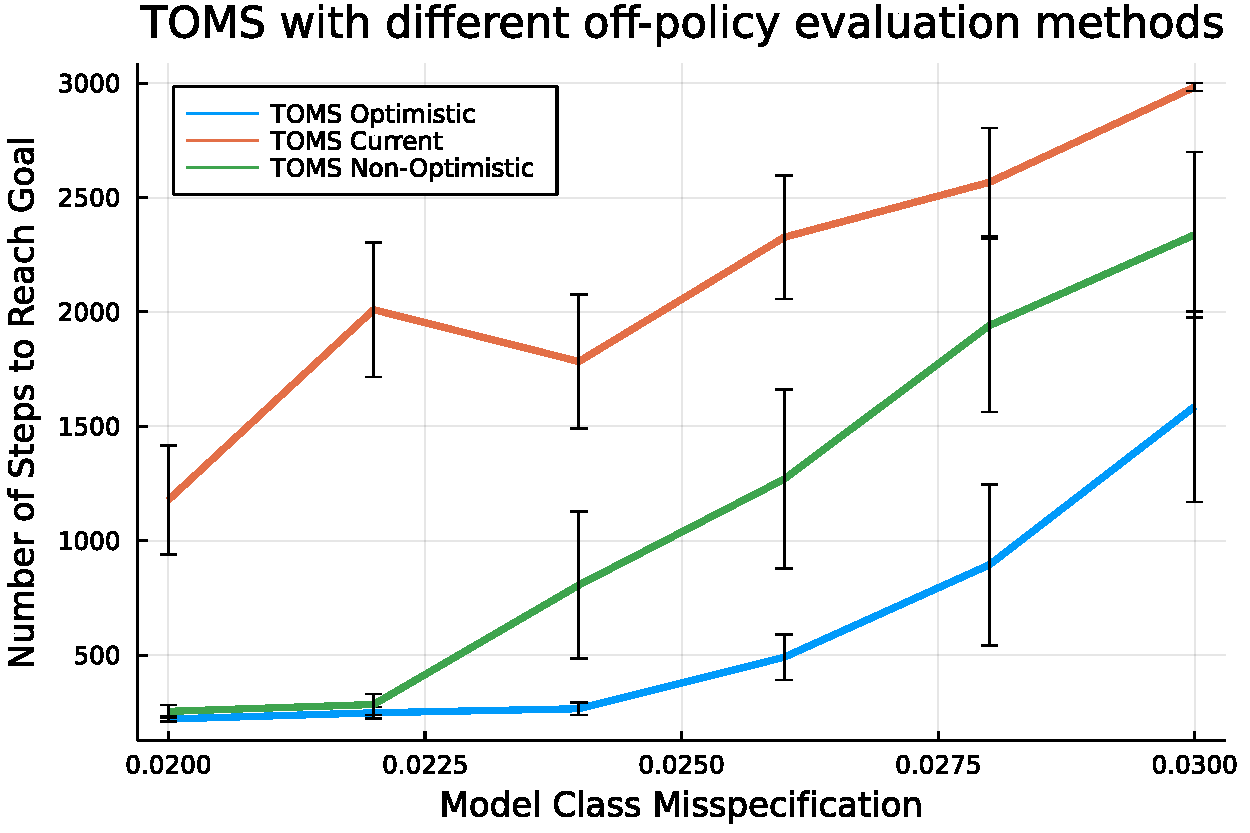
\includegraphics[width=0.5\linewidth]{figures/taml/mountain_car_online_model_search_toms.pdf}
  \caption{Performance versus misspecification on the mountain car
    domain. We compare \taml{} with different off-policy evaluation
    methods to understand if using optimistic evaluation helps it
    reach goal quickly}
  \label{fig:evaluation}
\end{figure}
\section{Discussion}
\label{sec:discussion-1}


  
%%% Local Variables:
%%% mode: latex
%%% TeX-master: "../main"
%%% End:
